\documentclass[a4paper]{article} 
\addtolength{\hoffset}{-2.25cm}
\addtolength{\textwidth}{4.5cm}
\addtolength{\voffset}{-3.25cm}
\addtolength{\textheight}{5cm}
\setlength{\parskip}{0pt}
\setlength{\parindent}{0in}

%----------------------------------------------------------------------------------------
%	PACKAGES AND OTHER DOCUMENT CONFIGURATIONS
%----------------------------------------------------------------------------------------

\usepackage{blindtext} % Package to generate dummy text
\usepackage{charter} % Use the Charter font
\usepackage[utf8]{inputenc} % Use UTF-8 encoding
\usepackage{microtype} % Slightly tweak font spacing for aesthetics
\usepackage[english]{babel} % Language hyphenation and typographical rules
\usepackage{amsthm, amsmath, amssymb} % Mathematical typesetting
\usepackage{float} % Improved interface for floating objects
\usepackage[final, colorlinks = true, 
            linkcolor = black, 
            citecolor = black]{hyperref} % For hyperlinks in the PDF
\usepackage{graphicx, multicol} % Enhanced support for graphics
\usepackage{xcolor} % Driver-independent color extensions
\usepackage{marvosym, wasysym} % More symbols
\usepackage{rotating} % Rotation tools
\usepackage{censor} % Facilities for controlling restricted text
\usepackage{listings, style/lstlisting} % Environment for non-formatted code, !uses style file!
\usepackage{pseudocode} % Environment for specifying algorithms in a natural way
\usepackage{style/avm} % Environment for f-structures, !uses style file!
\usepackage{booktabs} % Enhances quality of tables
\usepackage{tikz-qtree} % Easy tree drawing tool
\tikzset{every tree node/.style={align=center,anchor=north},
         level distance=2cm} % Configuration for q-trees
\usepackage{style/btree} % Configuration for b-trees and b+-trees, !uses style file!
\usepackage[backend=biber,style=numeric,
            sorting=nyt]{biblatex} % Complete reimplementation of bibliographic facilities
\addbibresource{ecl.bib}
\usepackage{csquotes} % Context sensitive quotation facilities
\usepackage[yyyymmdd]{datetime} % Uses YEAR-MONTH-DAY format for dates
\renewcommand{\dateseparator}{-} % Sets dateseparator to '-'
\usepackage{fancyhdr} % Headers and footers
\pagestyle{fancy} % All pages have headers and footers
\fancyhead{}\renewcommand{\headrulewidth}{0pt} % Blank out the default header
\fancyfoot[L]{} % Custom footer text
\fancyfoot[C]{} % Custom footer text
\fancyfoot[R]{\thepage} % Custom footer text
\newcommand{\note}[1]{\marginpar{\scriptsize \textcolor{red}{#1}}} % Enables comments in red on margin

%----------------------------------------------------------------------------------------

\usepackage{algorithmicx}
\usepackage{algorithm}
\usepackage{algpseudocode}
\usepackage{graphics}
\graphicspath{{./images/}}
\def\NoNumber#1{{\def\alglinenumber##1{}\State #1}\addtocounter{ALG@line}{-1}}
\begin{document}

%-------------------------------
%	TITLE SECTION
%-------------------------------

\fancyhead[C]{}
\hrule \medskip % Upper rule
\begin{minipage}{0.295\textwidth} 
\raggedright
\footnotesize
VO TRAN QUANG TUAN \hfill\\   
18127248\hfill\\
18127248@student.hcmus.edu.vn
\end{minipage}
\begin{minipage}{0.4\textwidth} 
\centering 
\large 
Homework Assignment 2\\ 
\normalsize 
Introduction To Design And Analysis Of Algorithms, Fall 2020\\ 
\end{minipage}
\begin{minipage}{0.295\textwidth} 
\raggedleft
\today\hfill\\
\end{minipage}
\medskip\hrule 
\bigskip

%-------------------------------
%	CONTENTS
%-------------------------------
\tableofcontents 
\newpage
%------------------------------------------------
\section{Problem 1}
Analyze the complexity of the function $Permutation()$ presented in Chapter 3: Brute-Force technique (Exhaustive Search section). \par
Pseudo code: \par
\begin{algorithm}
\renewcommand{\thealgorithm}{}
    \caption{Generate Permutations of Set A}
    
    \begin{algorithmic}[1]
    \Procedure{Permutations}{$pivot, a[1 \ldots n]$} \Comment{Generate the permutations of a, with a pivot}
        \If  {$pivot == n$}
            \State \Call{Print}{$a$};
        \Else
            \For {$i = pivot, \ldots, n$}
            \State \Call{Swap}{$a[pivot], a[i]$}
            \State \Call{Permutations}{$pivot+1, a$}
            \State \Call{Swap}{$a[pivot], a[i]$}
            \EndFor
        \EndIf
    \EndProcedure
        
    \end{algorithmic}

\end{algorithm}
Before analyzing the time complexity of $Permutations$ algorithm, we must determine some details:
\begin{itemize}
    \item The size of input: an pivot (don't care about that, it is an integer represents the position of each array's element to call the recursion), array input of $n$ numbers. So the size of input is $n$.
    \item Basic operations: the swap function between $a[pivot]$ and $a[i]$, also $a[i]$ and $a[pivot]$.
    \item The arrangement of input is not important because it doesn't affect to the time executes algorithm.
\end{itemize}
Let's denote T(n) is the number of times the basic operation is executed when running this algorithm. \par
Clearly, with $pivot=n$, the algorithm doesn't execute any swapping, so $T(1)=0$. \par
And what happen when $pivot != n$, slightly, we can see that this algorithm executes the for loop. In the for loop, we have two swapping and a recursion function involved. So with the for loop from $i=1$ to $i=n$, we have $2 \cdot n$ swapping and $2\cdot n \in \Theta(n) $, and $n \cdot T(n-1)$ times for involving the recursion:
\begin{gather*}
    T(n) = n \cdot T(n-1) + \Theta(n) \\
    T(1) = 0
\end{gather*}
To simplifying the $2 \cdot n$, we change it to $n$, because they belong to $ \Theta(n)$. \par
\begin{gather*}
    T(n) = n \cdot T(n-1)+n \\
    = n \cdot (n-1) \cdot T(n-2) + n \cdot (n-1) + n \\
    = n \cdot (n-1) \cdot (n-2) \cdot T(n-3) + n \cdot (n-1) \cdot (n-2) + n \cdot (n-1) + n \\
    \ldots \\
    = \frac{n!}{(n-i)!} \cdot T(n-i) + \frac{n!}{(n-1)!} +  \frac{n!}{(n-2)!} + \ldots + \frac{n!}{(n-i)!}
\end{gather*}
With the initial condition: $T(1) = 0$, let $n-i=1:$
\begin{gather*}
        T(n) = \frac{n!}{(n-i)!} \cdot T(n-i) + \frac{n!}{(n-1)!} +  \frac{n!}{(n-2)!} + \ldots + \frac{n!}{(n-i)!} \\
    = \frac{n!}{1!} \cdot 0 + \frac{n!}{(n-1)!} + \frac{n!}{(n-2)!} + \ldots + \frac{n!}{(1)!} \\ 
    = n! \cdot [\frac{1}{(1)!} + \frac{1}{(2!)} + \ldots + \frac{1}{(n-1)!}]
\end{gather*}
Taylor's Theorem: with $x \rightarrow 0$
\begin{equation*}
    e^x \approx 1 + \frac{x^1}{1!} + \frac{x^2}{2!} + \ldots + \frac{x^n}{n!}
\end{equation*}
So:
\begin{equation*}
    T(n) \geq n! \cdot e \implies T(n) \in \Omega (n!)
\end{equation*}
\newpage
%------------------------------------------------
\section{Problem 2}
A given boolean matrix $G[1..n, 1..n]$, where $n>3$, which is supposed to be adjacency matrix for a graph modeling a network with one of three topologies: Ring, Star and Fully connected mesh.\par
\begin{center}
    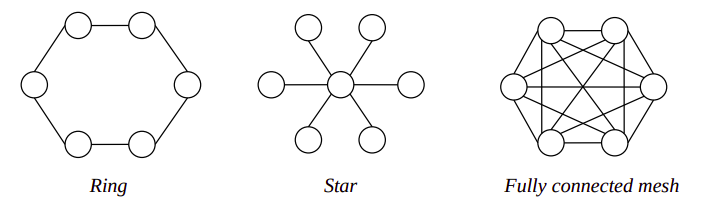
\includegraphics[scale=0.6]{image/problem2.png}
\end{center}
Obiviously, the adjacency matrix illustrate the connection between all vertices in a graph. each cell in this matrix represents number of edges between two particular vertex in graph correspond with the index of row and index of col in adjacency matrix. \par
Let's concentrate in the adjacency matrices which correspond with three kinds of graph in the picture above. Clearly, we can infer some comments from it:
\begin{itemize}
    \item With the Ring topology, degree of each vertex is exactly 2. So the sum of all value in each row or each column of the adjacency matrix is 2.
    \item With the Star topology, degree of each vertex is exactly 1 except an center vertex has degree $n-1$ with $n$ is numbers of vertex in this graph. So the sum of each row or each column ($n-1$ row or $n-1$ column except 1 column/1 row) in the adjacency matrix is 1, except 1 row/1 column has sum is $n-1.$
    \item With the fully connected mesh, clearly, we can see that each row/each column in the adjacency matrix has sum is $n-1$, because each vertex fully connects to the other vertices.
\end{itemize}
Following the analyzing above, we can design an brute-force algorithm for determine which kinds of topologies base on the adjacency matrix. \par
Pseudo code: \par
\begin{algorithm}
\renewcommand{\thealgorithm}{}
\caption{Which Topologies?}
\begin{algorithmic}[1]
\Procedure{Sum}{$A[1\ldots n]$}
    \State $S \gets 0$
    \For{$i=1, \ldots, n$}
        \State $S += A[i]$
    \EndFor
    \State \Return{$S$}
\EndProcedure
\State
\Procedure{SpecifyTopology}{$G[1 \ldots n, 1 \ldots n]$} \Comment{Specify the kind of topology corresponds with the adjacency matrix $G$}
    \State $i \gets 1$
        \If{\Call{Sum}{$G[i]$} $ == 2$} \Comment{$G[i]$ is row}
            \State \Return{$Ring$}
        \EndIf
        
        \If{\Call{Sum}{$G[i]$} $==n-1$ \AND \Call{Sum}{$G[i+1]$}$== n-1$}
            \State \Return{$Fully$ $connected$ $mesh$}
        \Else
            \State \Return{$Star$}
        \EndIf
\EndProcedure
\end{algorithmic}
\end{algorithm}
Let's analyzing the time complexity of this algorithm. To begin with the $Sum$ function, it calculates the sum of an array, so the time complexity of this function at each call step is $f(n) = n \in \Theta(n)$. \par
Next, we consider to the $SpecifyTopology$ function. The basic operation is in if conditions. Let $g(n)$ is the time complexity, with a specific adjacency matrix, all the if conditions in this algorithm were executed. So $g(n) = n + n + n = 3 \cdot n \in \Theta(n)$. So the time complexity is linear.
\newpage
%------------------------------------------------
\section{Problem 3}
Partition Problem: In number theory and computer science, the partition of problem is the task of deciding whether a given set $S$ of $n$ positive integers can be partitioned into two subset $S_1$ and $S_2$ such that the sum of the number in $S_1$ equals the sum of the numbers in $S_2$. With brute-force approach, a simple solution is that we can generate all the subset of the given set. \par
Pseudo code: \par
\begin{algorithm}
\renewcommand{\thealgorithm}{1}
\caption{Generate all Subset of Set A}
\begin{algorithmic}[1]
\Procedure{Subset}{$a[1 \ldots n]$}
    \State $Set \gets \{\emptyset\}$   
    \For{$i=1, \ldots, n$}
        \State $len \gets$ \Call{Length}{$Set$}
        \For{$j=1, \ldots, len$}
            \State $temp \gets Set[j]$
            \State $temp \gets temp \cup a[i] $
            \State $Set \cup temp$
        \EndFor
    \EndFor
    \State \Return{$Set$}
\EndProcedure
\end{algorithmic}
\end{algorithm}
After that, we calculate the sum of each subset and compare with the remaining set when use the except operator between the given set and current subset. \par
Pseudo code: \par
\begin{algorithm}
\renewcommand{\thealgorithm}{2}
\caption{Which set satisfies Partition Problem?}
\begin{algorithmic}
\Procedure{PartitionProblem}{$a[1 \ldots n]$}
    \State $Set \gets$ \Call{InitialSet}{$a$}
    \State $ListSubSet \gets$ \Call{Subset}{$a$}
    \For{$SubSet$ in $ListSubSet$}
        \If{\Call{Sum}{$SubSet$} $==$ \Call{Sum}{$Set \setminus SubSet$}}
        \State \Return{true}
        \EndIf
    \EndFor
    \State \Return{false}
\EndProcedure
\end{algorithmic}
\end{algorithm}

Let's analyzing the time complexity of this algorithm. Firstly, looking at the $SubSet(a)$ function, we can see that: 
\begin{itemize}
    \item The basic operation is the second assign operation in the for loop. Particularly, it is $temp \gets temp \cup a[i]$.
    \item Let $f(n)$ is the time complexity of this function: 
    \begin{itemize}
        \item $i=1, j=1 \implies$ loop $1=2^0$ time.
        \item $i=2, j \in [1, \ldots, 2^1] \implies$ loop $2^1$ times.
        \item $i=3, j \in [1, \ldots, 2^2] \implies$ loop $2^2$ times.
        \par
        \ldots
        \item $i=n, j \in [1, \ldots, 2^{n-1}] \implies$ loop $2^{n-1}$ times.
    \end{itemize}
    \item So, the time complexity:
    \begin{equation*}
        f(n) = \sum_{i=0}^{n-1}{2^i} = 2^n - 1 \in \Theta(2^n)
    \end{equation*}
\end{itemize}
Next, considering the $PartitionProblem(a)$ function, we can see that:
\begin{itemize}
    \item The basic operation is in the if condition in the for loop.
    \item Let $g(n)$ is the time complexity of this function, clearly $g(n) \in \Theta(n^2)$.
\end{itemize}
In conclusion, the time complexity for this partition problem with brute-force approach is $\Theta(max\{n^2,2^n\}) = \Theta(2^n)$
\newpage
%------------------------------------------------
\section{Problem 4}
A magic square of order n is an arrangement of $n^2$ numbers (from $1$ to $n^2$) in a square, such that the n numbers in all rows, all columns and both diagonals sum to the same constant t.
\subsection{Problem 4.a}
Prove that $t = \frac{n\cdot(n^2+1)}{2}$. \par
We have an arrangement of $n^2$ numbers (from $1$ to $n^2$), so the sum all of them is $\frac{n^2 \cdot (n^2+1)}{2}$.\par
But with the property of magic square, we have $n$ rows with the same sum, so: 
\begin{equation*}
    t = \frac{n^2 \cdot (n^2+1)}{2\cdot n} = \frac{n \cdot (n^2+1)}{2}
\end{equation*}
\subsection{Problem 4.b}
Generate all magic squares of order n with brute-force approach, we can generate all the permutations of the array $a[1 \ldots n^2]$, and check all sum in all rows, columns and diagonals. Compare with the $t$ in problem $4.a$. If existing one sum different from $t$, return false, else return true. \par
Firstly, Generate all the permutations of the array $a[1, \ldots, n^2]:$ \par
Pseudo code: \par
\begin{algorithm}
\renewcommand{\thealgorithm}{1}
    \caption{Generate Permutations of Set A}
    
    \begin{algorithmic}[1]
    \Procedure{Permutations}{$pivot, a[1 \ldots n], Set$} \Comment{Generate the permutations of a, with a pivot}
        \If  {$pivot == n$}
            \State $Set \cup a$ \Comment{Set contains all permutaions of a}
        \Else
            \For {$i = pivot, \ldots, n$}
            \State \Call{Swap}{$a[pivot], a[i]$}
            \State \Call{Permutations}{$pivot+1, a$}
            \State \Call{Swap}{$a[pivot], a[i]$}
            \EndFor
        \EndIf
    \EndProcedure
        
    \end{algorithmic}

\end{algorithm}
Secondly, calculate sum of row, column, diagonal and compare with $t$: \par
Pseudo code: \par
\begin{algorithm}
\renewcommand{\thealgorithm}{2}
\caption{Compare sum of each row, column, diagonal with t}
\begin{algorithmic}
\Procedure{Comparesum}{$A[1 \ldots n^2]$}
    \State $Matrix \gets$ \Call{CreateMatrix}{$A$}
    \For{$i=1, \ldots, n$} \Comment{Compare sum of row with $t$}
        \If{\Call{Sum}{$Matrix[i]$} $\neq t$}
        \State \Return{false}
        \EndIf
    \EndFor
    \State
    \State $SumCol \gets 0$
    \For{$i=1, \ldots, n$} \Comment{Compare sum of column with $t$}
        \For{$j=1, \ldots, n$}
            \State $SumCol \gets SumCol+Matrix[j][i]$
        \EndFor
        \If{$SumCol \neq t$}
            \State \Return{false}
        \EndIf
        \State $SumCol \gets 0$
    \EndFor
    \State
    \State $Principal \gets 0$
    \State $Secondary \gets 0$
    \For{$i=1, \ldots, n$} \Comment{Compare sum of two diagonals with $t$}
        \For{$j=0,\ldots, n$}
            \If{$i==j$}
                \State $Principal \gets Principal + Matrix[i][j]$
            \EndIf
            \If{$(i+j) == (n-1)$}
                \State $Secondary \gets Secondary + Matrix[i][j]$
            \EndIf
        \EndFor
    \EndFor
    \If{$Principal \neq t \OR Secondary \neq t$}
    \State \Return{false}
    \EndIf
    \State \Return{true}
\EndProcedure
\end{algorithmic}
\end{algorithm}
\newpage
Finally, checking each permutations of this array satisfy the property of magic square, if true, print the array. \par
Pseudo code: \par
\begin{algorithm}
\renewcommand{\thealgorithm}{3}
\caption{Generate all magic squares of order n}
\begin{algorithmic}
\Procedure{GenerateMagicSquare}{$n$}
    \If{$n==1$}
    \State \Call{Print}{$1$}
    \EndIf
    \If{$n==2$} 
    \State \Call{Print}{$\emptyset$}
    \EndIf
    \State $A \gets$ \Call{InitialArray}{n} \Comment{Initial array A with element belong to $1 \ldots n^2$}
    \State $Set \gets \{\}$
    \State \Call{Permutations}{$1, A, Set$}
    \For{$per$ in $Set$}
        \If{\Call{Comparesum}{$per$}} \Comment{Satisfy the property of magic square?}
        \State \Call{Print}{per}
        \EndIf
    \EndFor
\EndProcedure
\end{algorithmic}
\end{algorithm}
Let's analyzing the time complexity of this algorithm for this problem, let $f(n)$ is the time complexity of $GenerateMagicSquare$. With $Permutations$ function, we have $(n^2)!$ array, the time complexity is $\Omega((n^2)!)$, with the $Comparesum$ function, the time complexity is $\Theta(n^2)$. Looking carefully to the for loop in $GenerateMagicSquare$, we can see that the for execute $(n^2)!$ times. So:
\begin{equation*}
    f(n) = n^2 \cdot (n^2)!  \in \Theta(n^2 \cdot (n^2)!)
\end{equation*}

\newpage
%------------------------------------------------
\end{document}
